\section{Gestion de versions du code source}
\label{section:pic-source}

\paragraph{}
La gestion de versions du code source est l'outil de prédilection d'une équipe de développement agile.
En effet, elle permet de suivre l'ensemble des modification effectuées sur le code de façon incrémentale.
Par ailleurs, il faut noter qu'elle ne se borne pas au versionnement de code source.
Il est ainsi possible de stocker dans un dépôt tout ficher texte, mais aussi tout fichier binaire (e.g. images, documents Office, etc.).

\paragraph{}
En pratique, à chaque fois qu'un fichier est ajouté au dépôt\footnote{Un dépôt est l'endroit virtuel où sont stockés les fichiers source.} ou qu'il est modifié, son état courant est sauvegardé de façon à pouvoir éventuellement être récupéré plus tard.
Ces versions gelées prennent le nom de \emph{révisions}.
Elles sont dotées d'un identifiant -- qui peut être un simple numéro ou bien un hash\footnote{On nomme fonction de hachage une fonction particulière qui, à partir d'une donnée fournie en entrée, calcule une empreinte servant à identifier rapidement, bien qu'incomplètement, la donnée initiale.~\cite{hash}} -- et contiennent un certain nombre d'informations utiles comme le nom et l'adresse e-mail de l'auteur, la date de création, un message descriptif des changements, etc.
En outre, on appelle \acommit{} l'action de créer une révision.

\paragraph{}
L'utilisation d'un système de gestion de versions apporte de nombreux avantages.
En effet, la pratique ancestrale consiste à copier l'ensemble du code source de l'application manuellement, soit à des points clés du cycle de développement -- comme les jalons par exemple -- soit de manière sporadique -- au bon vouloir des chefs de projet et des développeurs.
Pour le coup, une telle méthode est tout à fait inefficace du point de vue qu'elle est régulièrement soumise à des erreurs humaines, et qu'elle est abusivement consommatrice en espace de stockage alors que les différences entre les sauvegardes peuvent être très limitées.

Au contraire, la gestion de versions donne la possibilité d'automatiser de tels processus, permettant ainsi d'aider à tendre vers une industrialisation du développement logiciel.
Les deux inconvénients de la sauvegarde traditionnelle cités précédemment sont résolus, car le versionnement régulier est favorisé et car le stockage des révisions se fait de manière incrémentale, respectivement.

De plus, il devient possible de travailler de manière vraiment collaborative : plusieurs développeurs peuvent travailler sur les même fichiers source sans pour autant se gêner les uns les autres.
Dans le cas où une même portion de code est modifiée par plusieurs personnes, un conflit est détecté et doit être résolu manuellement : c'est une simple étape complètement intégrée au processus.

Un outil de gestion de versions facilite également la résolution de bugs, en permettant de naviguer aisément entre les différentes versions de fichiers source.
Étant donné que la granularité des changements entre deux révisions consécutives est relativement fine, on peut détecter l'instant précis où un bug a été introduit et éventuellement annuler les changements de la révision impliquée.

Enfin, la gestion de versions permet de réduire les appréhensions liées au développement de nouvelles fonctionnalités expérimentales.
Partir dans un nouveau développement indépendant alors que des changements doivent toujours être effectués sur une version dite stable -- celle en production par exemple -- ne pose plus problème.
Les outils donnent la possibilité de fusionner des bases de code qui ont évolué de façon distincte -- appelée \emph{branches} -- par le même système de gestion des conflits qui a été cité précédemment.

\paragraph{}
Versionner le code source de son logiciel n'apporte donc que des avantages.
La seule contrepartie réside dans le fait que les développeurs doivent être formés à l'outil choisi et motivés par son utilisation.
En effet, en tant que premiers utilisateurs du système, ils doivent en voir les bénéfices pour appliquer les bonnes pratiques inhérentes.

\paragraph{}
L'ensemble du jargon spécifique à la gestion de version qui a été évoqué dans cette section est illustré en \reffigure{pic-source:jargon-depot} et en \reffigure{pic-source:jargon-branches}.

\begin{figure}
	\centering
	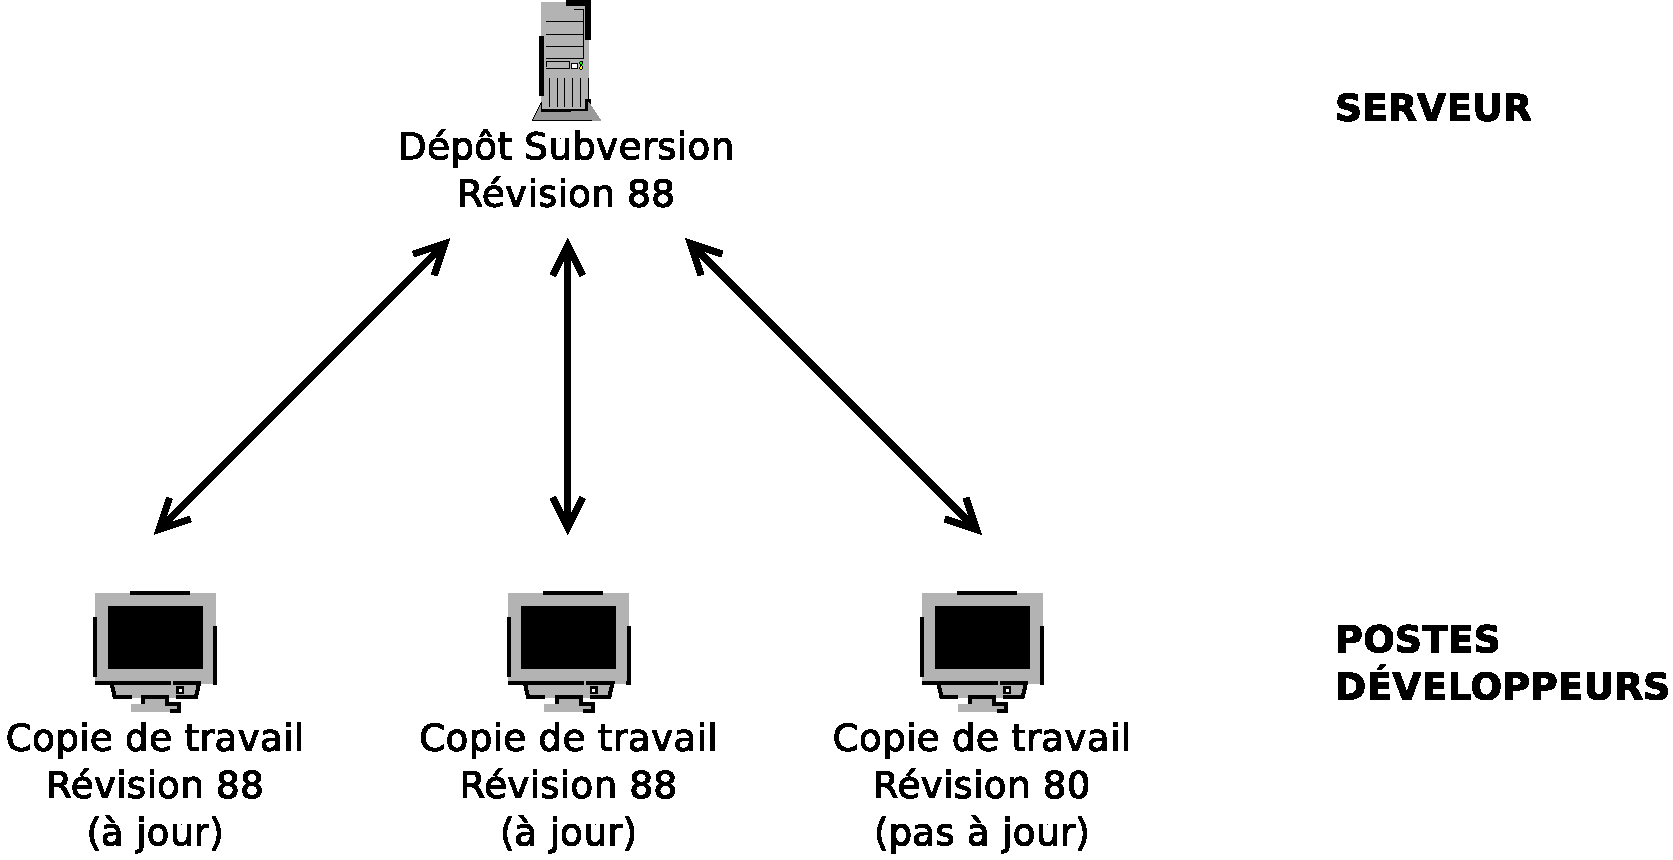
\includegraphics[width=12cm]{pic/jargon-depot}
	\caption{Illustration des concepts de dépôt et de copie de travail}
	\label{figure:pic-source:jargon-depot}
\end{figure}

\begin{figure}
	\centering
	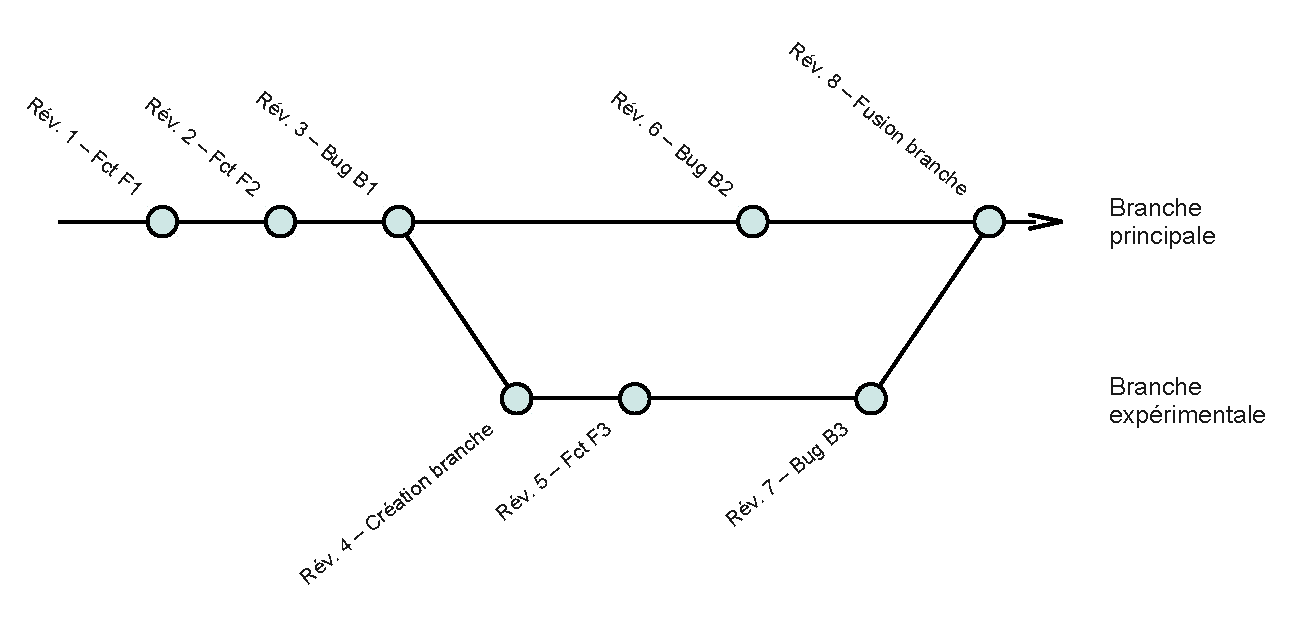
\includegraphics[width=14cm]{pic/jargon-branches}
	\caption{Illustration des concepts de révisions et de branches}
	\label{figure:pic-source:jargon-branches}
\end{figure}



\subsection{Outils}

\subsubsection{Subversion}

\paragraph{}
Subversion, souvent abrégé SVN, est certainement l'outil open source de gestion de versions le plus répandu dans les entreprises aujourd'hui.
Malgré l'apparition relativement récente de plusieurs solutions concurrentes, il reste encore massivement utilisé par les communautés open source pour gérer le code de leurs projets.


\paragraph{}
Il permet une gestion de versions dite \emph{centralisée}.
Cela implique qu'il n'existe qu'un seul dépôt de référence répertoriant l'ensemble des révisions.
Chaque développeur utilise un client Subversion afin de récupérer une \emph{copie de travail} locale du projet.
Il peut ensuite envoyer ses modifications des fichiers au dépôt sous la forme de révisions, à la seule condition que la copie de travail soit à jour.

Le modèle centralisé donne l'avantage d'être simple à appréhender, c'est le plus répandu dans le monde professionnel du fait de sa maturité.
Néanmoins, son inconvénient réside le fait que toutes les révisions soient stockées uniquement sur le dépôt.
Si ce dernier n'est plus accessible, les clients de l'outil ne sont pas capables d'être autonomes et ne peuvent plus remplir leurs fonctions.

À ce modèle on oppose la gestion de versions dite \emph{décentralisée} qui, elle, implique qu'il n'y ait pas de dépôt unique répertoriant l'ensemble de révisions.
En fait, chaque copie de travail est un dépôt à part entière contenant toutes révisions et que l'on synchronise régulièrement avec le dépôt considéré comme \og principal \fg.



\subsection{Missions}

\subsubsection{Formation Subversion chez Rexel}

Au même titre que la formation JIRA, j'ai également pu participer au début de mon stage à la formation Subversion donnée chez Rexel par \agulet.
Je connaissais déjà très bien l'outil, j'ai principalement appris de la façon de le présenter à un client.



\subsubsection{Proposition d'architecture Subversion pour Rexel}

Rexel possédait déjà un certain nombre de dépôts SVN dont l'architecture avait été mise en place par \asmile.
Externalisant la plupart du temps ses tâches de développement, le client souhaitait trouver une solution dans le cas où le prestataire de service désire travailler sur son propre dépôt SVN chez lui en interne.
Avec \agulet, nous avons fait plusieurs propositions de solutions :
\begin{itemize}
	\item utiliser un système de miroirs de dépôts -- Rexel posséderait alors un dépôt miroir en lecture seule de celui du prestataire ;
	\item le prestataire développe sur son propre dépôt, et à chaque livraison une révision est créée sur le dépôt de Rexel qui reste indépendant ;
	\item migrer vers un système de gestion de versions décentralisé.
\end{itemize}

Finalement, le client n'a pas donné suite à nos propositions et a conservé son système en l'état.

